\documentclass[12pt]{article}

\usepackage{amsmath,amsthm,amsfonts,amssymb,amsxtra}
\usepackage{pgf,tikz}
\usetikzlibrary{arrows}
\renewcommand{\theenumi}{(\alph{enumi})} 
\renewcommand{\labelenumi}{\theenumi}

\pagestyle{empty}
\setlength{\textwidth}{7in}
\setlength{\oddsidemargin}{-0.5in}
\setlength{\topmargin}{-1.0in}
\setlength{\textheight}{9.5in}

\theoremstyle{definition}
\newtheorem{problem}{Problem}

\begin{document}

\noindent{\large\bf MATH 241}\hfill{\large\bf Final Exam.}\hfill{\large\bf
  Spring 2018}\hfill{\large\bf Page 1/8}\hrule

\bigskip
\begin{center}
  \begin{tabular}{|ll|}
    \hline & \cr
    {\bf Name: } & \makebox[12cm]{\hrulefill}\cr & \cr
    {\bf VIP ID:} & \makebox[12cm]{\hrulefill}\cr & \cr
    \hline
  \end{tabular}
\end{center}
\begin{itemize}
\item Write your name and your VIP ID in the space provided above.
\item The test has nine (9) pages, including this one, and the formula sheet attached at the end. 
\item You have 150 minutes to complete this test.
\item Each problem is worth 10 points.
\item Enter your answer in the box(es) provided.
\item You must show sufficient work to justify all answers unless otherwise stated in the problem.  Correct answers with inconsistent work may not be given credit.
\item No books, notes or calculators may be used on this test.
\end{itemize}
\hrule

 \begin{center}
   \begin{tabular}{|c|c|c|}
     \hline
     &&\cr
     {\large\bf Page} & {\large\bf Max} & {\large\bf Points} \cr
     &&\cr
     \hline
     &&\cr
     {\Large 2} & \Large 20 & \cr
     &&\cr
     \hline
     &&\cr
     {\Large 3} & \Large 20 & \cr
     &&\cr
     \hline
     &&\cr
     {\Large 4} & \Large 20 & \cr
     &&\cr
     \hline
     &&\cr
     {\Large 5} & \Large 10 & \cr
     &&\cr
     \hline
     &&\cr
     {\Large 6} & \Large 10 & \cr
     &&\cr
     \hline
     &&\cr
     {\Large 7} & \Large 10 & \cr
     &&\cr
     \hline
     &&\cr
     {\Large 8} & \Large 10 & \cr
     &&\cr
     \hline\hline
     &&\cr
     {\large\bf Total} & \Large 100 & \cr
     &&\cr
     \hline
   \end{tabular}
   \end{center}
\newpage

%%%%%%%%%%%%%%%%%%%%%%%%%%%%%%%%%%%%% Page 2
\noindent{\large\bf MATH 241}\hfill{\large\bf Final Exam.}\hfill{\large\bf
  Spring 2018}\hfill{\large\bf Page 2/8}\hrule

\bigskip
\begin{problem}
Find the distance from the point $(-4,-2,1)$ to the line $L$ with parametric equations
\begin{equation*}
L : \begin{cases}
x = 5 -t \\
y = 1 - 2t \\
z = -6 + 3t
\end{cases}
\end{equation*}
\vspace{6cm}
\begin{flushright}
  \begin{tikzpicture}
    \draw (-0.5cm,0.5cm) node {$d=$};
    \draw (0cm,-0.2cm) rectangle (10cm,1.2cm);
  \end{tikzpicture}
\end{flushright}
\end{problem}
\hrule
\begin{problem}[10 pts]
Find the intersection of the plane $x+y+z=-3$ with the line
\begin{equation*}
L : \begin{cases}
x = 3 + 2t \\
y = -3 + 4t \\
z = -3 + 6t
\end{cases}
\end{equation*}
\vspace{6cm}
\begin{flushright}
  \begin{tikzpicture}
    \draw (-1.25cm,0.5cm) node {Intersection:};
    \draw (0cm,-0.2cm) rectangle (10cm,1.2cm);
  \end{tikzpicture}
\end{flushright}
\end{problem}
\newpage

%%%%%%%%%%%%%%%%%%%%%%%%%%%%%%%%%%%%% Page 3
\noindent{\large\bf MATH 241}\hfill{\large\bf Final Exam.}\hfill{\large\bf
  Spring 2018}\hfill{\large\bf Page 3/8}\hrule

\bigskip
\begin{problem}
Consider the helix obtained as the graph of the following vector function 
\begin{equation*}
\boldsymbol{r}(t) = \cos \big(\tfrac{t}{2}\big) \boldsymbol{i} + \sin \big( \tfrac{t}{2} \big) \boldsymbol{j} +\tfrac{t}{2} \boldsymbol{k}.
\end{equation*}
\begin{enumerate}
  \item (5 pts) Prove that this helix lies on the cylinder $x^2+y^2=1$.
  \vspace{3cm}
  \item (5 pts) Calculate the length of the section of the helix for $0 \leq t \leq 4\pi$.
  \vspace{4cm}
  \begin{flushright}
    \begin{tikzpicture}
      \draw (-0.5cm,0.5cm) node {$\ell =$};
      \draw (0cm,-0.2cm) rectangle (10cm,1.2cm);
    \end{tikzpicture}
  \end{flushright}
\end{enumerate}
\end{problem}
\hrule
\begin{problem}[10 pts]
Find and sketch the domain of the function $f(x,y) = \sqrt{\strut y-6x-5}$

\vspace{1cm}
\begin{tikzpicture}[scale=0.9]
  \draw [white] (-0.5,-0.5) rectangle (6.5,6.5);
  \draw [<->, ultra thick] (-0.5,3) -- (6.5,3);
  \draw [<->, ultra thick] (3,-0.5) -- (3,6.5);
  \draw[step=0.5,gray,ultra thin] (-0.25, -0.25) grid (6.25, 6.25);
\end{tikzpicture}
\vspace{1cm}  
\begin{flushright}
  \begin{tikzpicture}
    \draw (0cm,0.5cm) node {The domain is};
    \draw (1.5cm,-0.2cm) rectangle (15cm,1.2cm);
  \end{tikzpicture}
\end{flushright}
\end{problem}
\newpage

%%%%%%%%%%%%%%%%%%%%%%%%%%%%%%%%%%%%% Page 4
\noindent{\large\bf MATH 241}\hfill{\large\bf Final Exam.}\hfill{\large\bf
  Spring 2018}\hfill{\large\bf Page 4/8}\hrule

\bigskip
\begin{problem}[10 pts]
Find all the local maxima, local minima and saddle points of the function 
\begin{equation*}
f(x,y) = x^3+y^3+3x^2-9y^2-1.
\end{equation*}
  \vspace{13cm}
\end{problem}
\hrule
\begin{problem}[10 pts]
Evaluate $\int_C \, (xy+y+z)\, ds$ along the curve $\boldsymbol{r}(t) = 2t \boldsymbol{i} +t \boldsymbol{j} + (6-2t) \boldsymbol{k}$, for $0 \leq t \leq 1$.
\vspace{5cm}
\begin{flushright}
  \begin{tikzpicture}
    \draw (-2cm,0.5cm) node {$\displaystyle{\int_C \, (xy+y+z)\, ds=}$};
    \draw (0cm,-0.2cm) rectangle (5cm,1.2cm);
  \end{tikzpicture}
\end{flushright}
\end{problem}
\newpage

%%%%%%%%%%%%%%%%%%%%%%%%%%%%%%%%%%%%% Page 5
\noindent{\large\bf MATH 241}\hfill{\large\bf Final Exam.}\hfill{\large\bf
  Spring 2018}\hfill{\large\bf Page 5/8}\hrule

\bigskip
\begin{problem}[10 pts]
Find the absolute maximum and minimum (location and value) of the function $f(x,y) = 2x^2-4x+y^2-6y+3$ on the closed triangular region bounded by the lines $x=0$, $y=3$, $y=3x$ in the first quadrant.  Sketch the region.

\vspace{0.5cm}
\begin{tikzpicture}[scale=0.7]
  \draw [white] (-0.5,-0.5) rectangle (6.5,6.5);
  \draw [<->, ultra thick] (-0.5,0) -- (6.5,0);
  \draw [<->, ultra thick] (0,-0.5) -- (0,6.5);
  \draw[step=0.5,gray,ultra thin] (-0.25, -0.25) grid (6.25, 6.25);
  \end{tikzpicture}
\vspace{14cm}
\begin{flushright}
  \begin{tikzpicture}
    \draw (0cm,0.5cm) node {Maximum:};
    \draw (1.2cm,-0.2cm) rectangle (7.2cm,1.2cm);
    \draw (9cm,0.5cm) node {Minimum:};
    \draw (10.2cm,-0.2cm) rectangle (16.2cm,1.2cm);
  \end{tikzpicture}
\end{flushright}
\end{problem}
\newpage

%%%%%%%%%%%%%%%%%%%%%%%%%%%%%%%%%%%%% Page 6
\noindent{\large\bf MATH 241}\hfill{\large\bf Final Exam.}\hfill{\large\bf
  Spring 2018}\hfill{\large\bf Page 6/8}\hrule

\bigskip
\begin{problem}[10 pts]
Sketch the domain of integration, convert the polar integral to a Cartesian integral, and evaluate
\begin{equation*}
\int_{0}^{\pi/4} \int_{0}^{3\sec \theta} r^5 \sin^2\theta \, dr\, d\theta
\end{equation*}
\vspace{0.5cm}
\begin{tikzpicture}[scale=0.7]
  \draw [white] (-0.5,-0.5) rectangle (6.5,6.5);
  \draw [<->, ultra thick] (-0.5,0) -- (6.5,0);
  \draw [<->, ultra thick] (0,-0.5) -- (0,6.5);
  \draw[step=0.5,gray,ultra thin] (-0.25, -0.25) grid (6.25, 6.25);
  \end{tikzpicture}
\vspace{12cm}
\begin{flushright}
  \begin{tikzpicture}
    \draw (0cm,0.5cm) node {$\displaystyle{\int_{0}^{\pi/4} \int_{0}^{3\sec \theta} r^5 \sin^2\theta \, dr\, d\theta}=$};
    \draw (3cm,-0.3cm) rectangle (11.5cm,1.3cm);
    \draw (12cm,0.5cm) node {$=$};
    \draw (12.5cm,-0.3cm) rectangle (15cm,1.3cm);
  \end{tikzpicture}
\end{flushright}
\end{problem}
\newpage

%%%%%%%%%%%%%%%%%%%%%%%%%%%%%%%%%%%%% Page 7
\noindent{\large\bf MATH 241}\hfill{\large\bf Final Exam.}\hfill{\large\bf
  Spring 2018}\hfill{\large\bf Page 7/8}\hrule

\bigskip
\begin{problem}[10 pts]
Sketch the domain of integration, reverse the order of integration and evaluate
\begin{equation*}
\int_{0}^{2\sqrt{\ln 10}} \int_{y/2}^{\sqrt{\ln 10}} 8e^{x^2}\, dx\, dy
\end{equation*}
\vspace{0.5cm}
\begin{tikzpicture}[scale=0.7]
  \draw [white] (-0.5,-0.5) rectangle (6.5,6.5);
  \draw [<->, ultra thick] (-0.5,0) -- (6.5,0);
  \draw [<->, ultra thick] (0,-0.5) -- (0,6.5);
  \draw[step=0.5,gray,ultra thin] (-0.25, -0.25) grid (6.25, 6.25);
  \end{tikzpicture}
\vspace{12cm}
\begin{flushright}
  \begin{tikzpicture}
    \draw (0cm,0.5cm) node {$\displaystyle{\int_{0}^{2\sqrt{\ln 10}} \int_{y/2}^{\sqrt{\ln 10}} 8e^{x^2}\, dx\, dy}=$};
    \draw (3cm,-0.3cm) rectangle (11.5cm,1.3cm);
    \draw (12cm,0.5cm) node {$=$};
    \draw (12.5cm,-0.3cm) rectangle (15cm,1.3cm);
  \end{tikzpicture}
\end{flushright}
\end{problem}
\newpage

%%%%%%%%%%%%%%%%%%%%%%%%%%%%%%%%%%%%% Page 8
\noindent{\large\bf MATH 241}\hfill{\large\bf Final Exam.}\hfill{\large\bf
  Spring 2018}\hfill{\large\bf Page 8/8}\hrule

\bigskip
\begin{problem}[10 pts]
We want to find the volume of the solid bounded above by the sphere $x^2+y^2+z^2=360$ and below by the paraboloid $2z = x^2+y^2$. Sketch that solid, find an integral expression that computes its volume (double or triple integral, your choice), and evaluate that integral to obtain that volume.
\vspace{19cm}
\begin{flushright}
  \begin{tikzpicture}
    \draw (-3.25cm, 0.5cm) node {$\displaystyle{V = \iint_D f(x,y) dA = \iiint_R dV = }$};
    \draw (0cm,-0.2cm) rectangle (5cm,1.2cm);
  \end{tikzpicture}
\end{flushright}
\end{problem}

\end{document}
